\chapter{Introduction}
\label{chapter_introduction}

%% Start the actual chapter on a new page.
\newpage

\noindent 
\dropcap{S}{peciation} is the process that creates new species,
connecting all of life to one shared common ancestor. This process
can be investigated on multiple levels, for example at the individuals'
or at the species level. In this thesis, I focus on the latter.

Speciation at the species level simplifies a species to a horizontal 
line (also called a 'branch') in a phylogeny, answering
basic questions like 'Which species lived when?', 'When did a speciation 
event take place?' and 'Who is the ancestor of which species?'. 
Figure \ref{fig:phylogeny} shows an example phylogeny:

\begin{figure}[H]
  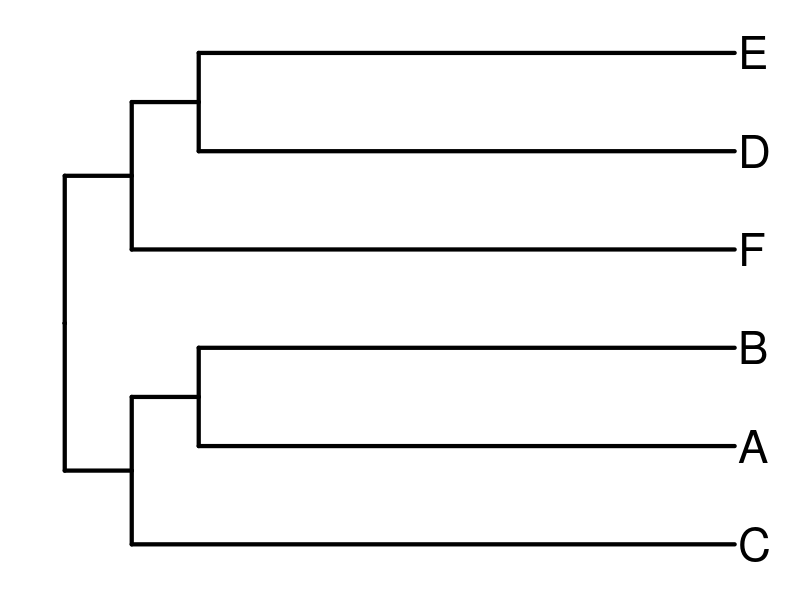
\includegraphics[width=0.4\textwidth]{phylogeny.png}
  \caption{
    A phylogeny with six species
  }
  \label{fig:phylogeny}
\end{figure}

Figure \ref{fig:phylogeny} shows a phylogeny (also called 'phylogenetic tree', 
or simply 'tree') with six hypothetical species and their evolutionary 
relationships. Going from left to right, we go from the past to the present 
time. The leftmost vertical line indicates the first speciation event, called
the crown age, which gave rise to the first two ancestral species. Each
of these ancestral species gives rise to its own evolutionary history,
resulting in a tree with two clades: the ABC and the DEF clades.

Phylogenies cannot be measured directly, as they depict which species lived
when \emph{in the past}. Even with a time machine, we would have a hard time
to observe when a speciation event took place. In the present, however, we
do have species that carry their own evolutionary history with them, in the
form of DNA. From the species we are interested in, 
we can obtain (part of) their DNA sequences. DNA sequences of different species 
may vary in length, due to insertions and deletions in genetic sequences.
Usually, we use a procedure (a software tool, for example) to align 
the sequences, as shown in figure \ref{fig:alignment}:

\begin{figure}[H]
  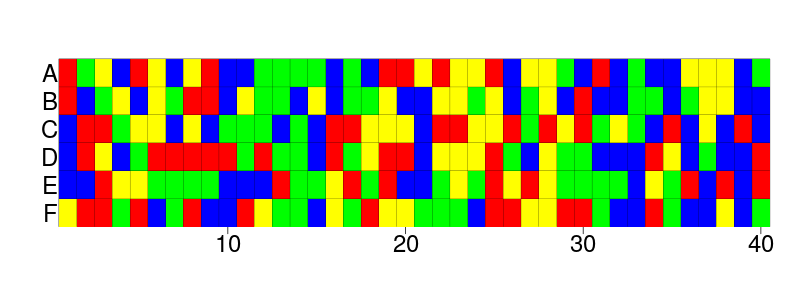
\includegraphics[width=0.8\textwidth]{alignment_40.png}
  \caption{
    A 40-nucleotide DNA alignment of the six species
  }
  \label{fig:alignment}
\end{figure}

Figure \ref{fig:alignment} shows an alignment of our six hypothetical species
that we actually could have found in nature. From this alignment, we
can \emph{infer} a phylogeny, which basically means 'best guess following a 
rational procedure'. There are multiple ways to infer a phylogeny, for
example, using maximum likelihood or Bayesian inference. In this thesis, 
I focus on the latter.

With Bayesian inference, we use an alignment and our model assumptions to infer 
a posterior (more 
precise: 'a joint posterior distribution of phylogenies and model parameters').
A posterior contains multiple inferred phylogenies, in which the more likely
ones are present more often. This distribution of phylogenies shows the
(un)certainty of the inference. Figure \ref{fig:densitree} shows the
posterior phylogenies we obtain from our alignment:

\begin{figure}[H]
  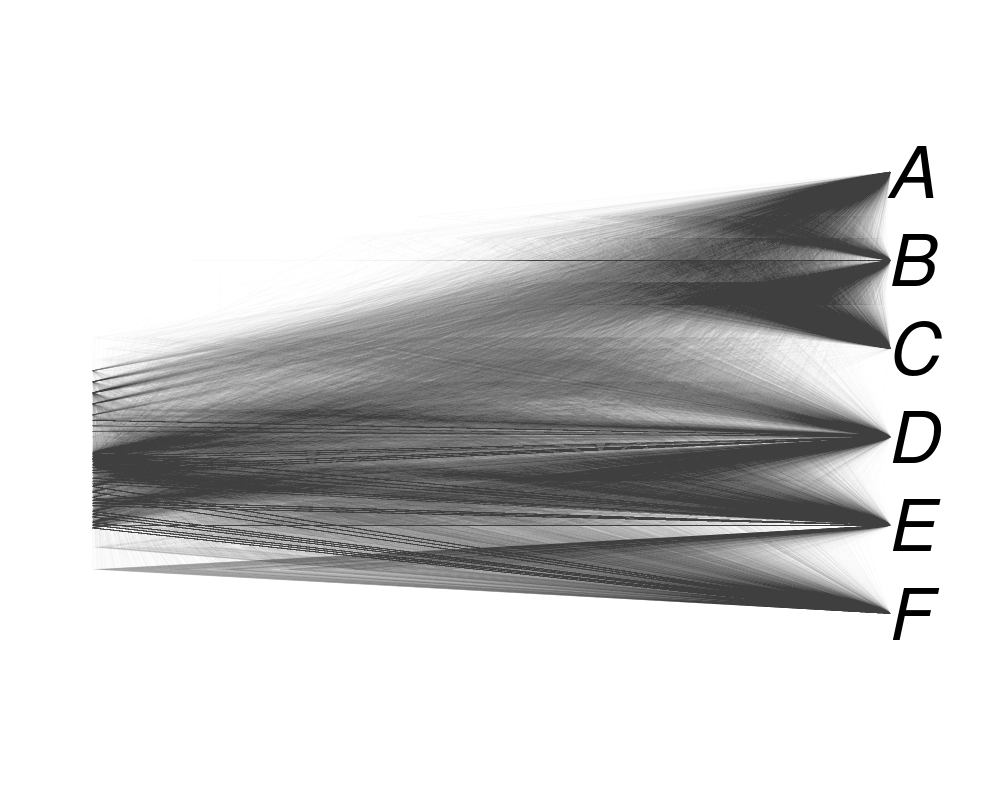
\includegraphics[width=0.8\textwidth]{densitree_40.png}
  \caption{
    The posterior phylogenies of the six species, 
    from a DNA alignment of 40 nucleotides
  }
  \label{fig:densitree}
\end{figure}

Figure \ref{fig:densitree} shows a high degree of uncertainty, as the
inferred phylogenies vary widely in shape. The inference only
weakly distinguishes between the ABC and DEF clades. 

The inference described so far is unsatisfactory, as we can only draw 
weak conclusions. We can improve the inference by using a longer DNA sequence 
or by picking a better inference model. In a simulation study, we can
easily increase the number of nucleotides, 
figure \ref{fig:densitree_again} shows the
posterior phylogenies we obtain from our longer alignment:

\begin{figure}[H]
  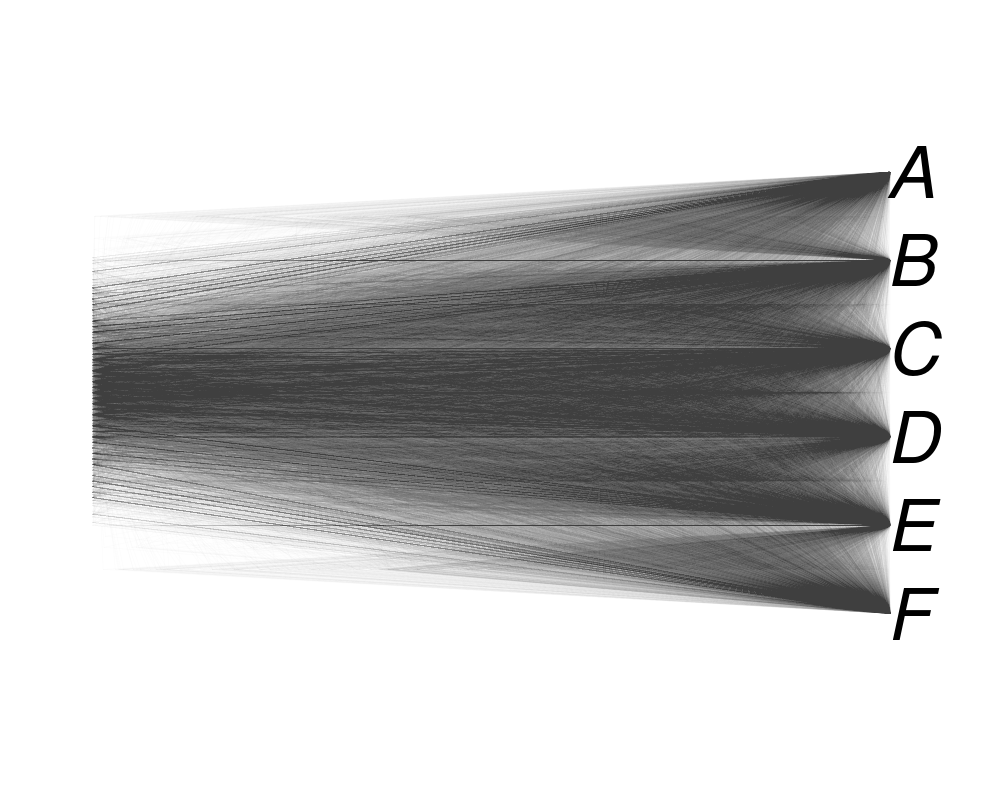
\includegraphics[width=0.8\textwidth]{densitree_400.png}
  \caption{
    The posterior phylogenies of the six species,
    from a DNA alignment of 400 nucleotides
  }
  \label{fig:densitree_again}
\end{figure}

Figure \ref{fig:densitree_again} shows that in this example,
with more information, we can only show our uncertainty more clearly. 

Another way to improve our inference is using a better inference model.
An inference model embodies our assumptions on how we think evolution
works, and consists of (1) how nucleotides mutate to others (also
called 'the site model'), (2) how often mutations occur (also 
called 'the clock model'), and (3) how speciation works (also 
called 'the tree prior' or 'the speciation model'). 
Theory predicts that usually the inference model becomes less important
if there is more information in an alignment. The example shows here,
however, shows one of the exceptions.

Ideally, we pick an inference model identical to the actual way things 
work (or: 'the true model'), be it in nature
or \textit{in silico}. In practice, the true model that nature uses is unknown.
Due to this, scientists came up with many models to explain the 
DNA (RNA, protein, morpholical and fossil) data best.

In a theoretical study, when can simply pick how nature works; that is,
how it is simulated. Theoretical studies are useful, as these explore
how well we will ever be able to explain nature. To do so, a 'true' 
speciation model is picked to generate 'true' phylogenies. 
From these phylogenies, a 'true' site model and clock model are used to
simulate a 'true' alignment. From that 'true' alignment, which is the
data we can gather from nature, we can then see how close our inferred
phylogenies are to the 'true' phylogeny.


There are many ways to quantify how similar two phylogenies are,
as phylogenies are complex structures. A summary statistic puts
a certain aspect of a tree into one or more numbers, for example,
the nLTT statistic [Janzen et al., ?] 

Simple examples are 

(in this
case, the known 'true' phylogeny and an inferred posterior
of phylogenies needs to be quantified, to know how well the inference

can be quantified using an error statistic. One way to
do so, is to take the error between two summary statistics. A summary
statistic summarizes part of the information embedded within a tree to
one or more values. Examples are the $\gamma$ statistic to ... and
the nLTT statistic . The latter we use ...

\begin{figure}[H]
  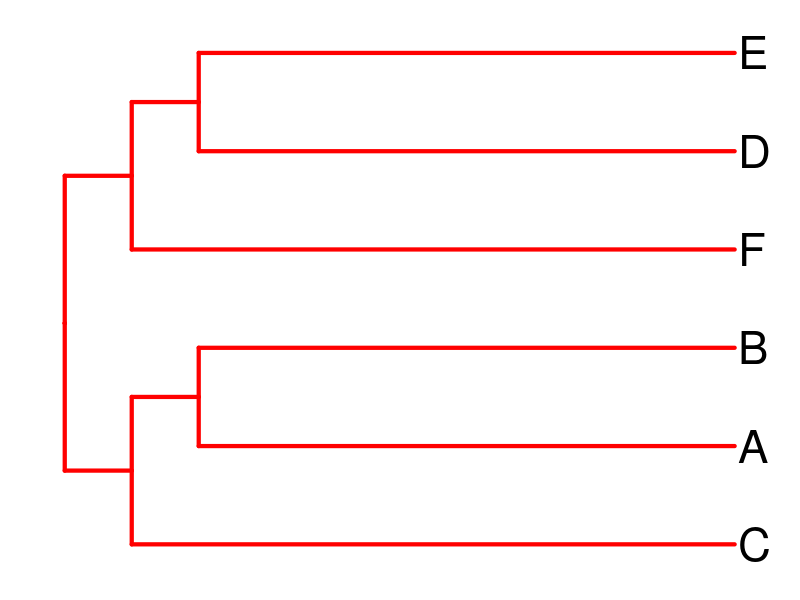
\includegraphics[width=0.8\textwidth]{true_tree.png}
  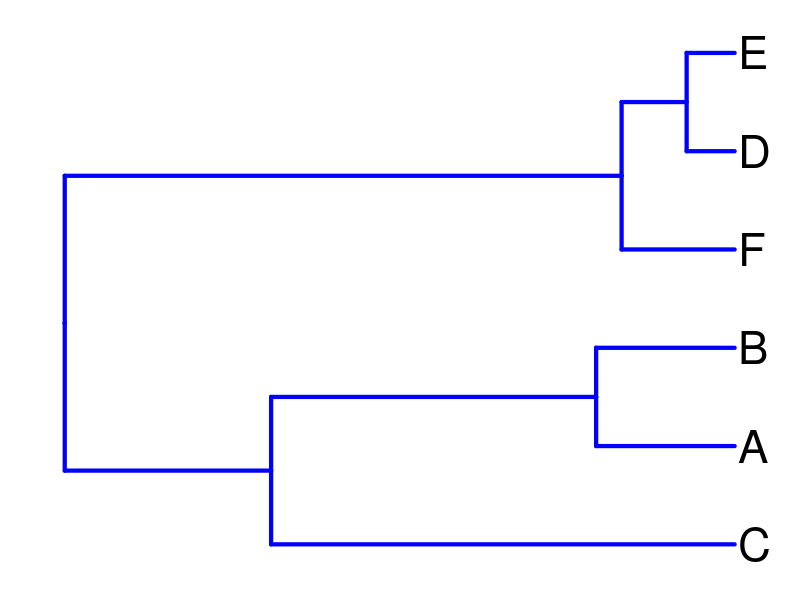
\includegraphics[width=0.8\textwidth]{twin_tree.png}
  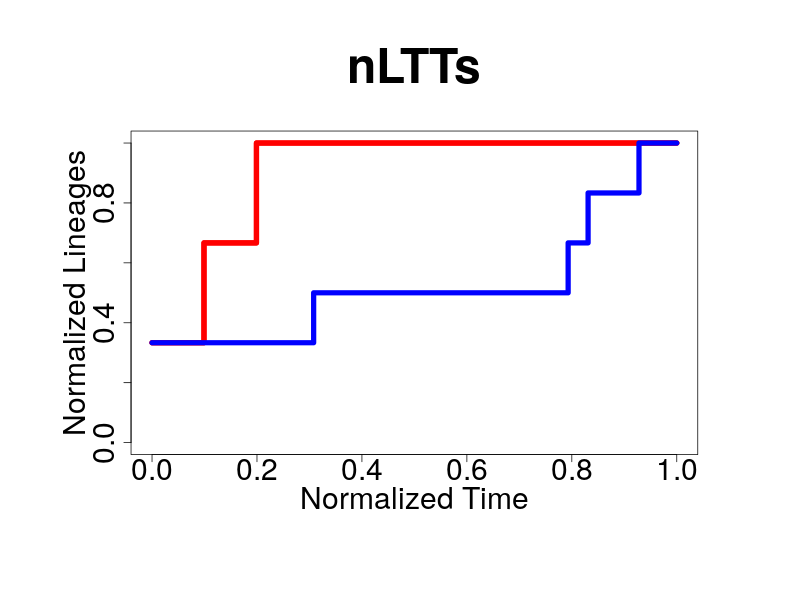
\includegraphics[width=0.8\textwidth]{nltt.png}
  \caption{
    nLTTs
  }
  \label{fig:densitree_again}
\end{figure}






There are many papers about which model works best on which data.
 



%\references{dissertation}

